\section{Technology comparison}

\begin{frame}{ADEV@1s vs. Size}

    Empirical correlation\footnotemark[1]: $\sigma_y(\tau=1) = 6.85 \times 10^{-10} + \text{volume}^{-0.64}$

    \begin{columns}[c, onlytextwidth]

        \begin{column}{0.7\textwidth}

            \begin{figure}
                \centering
                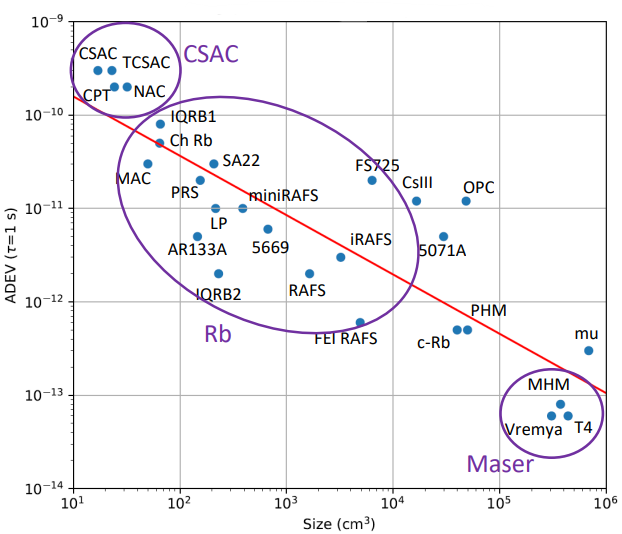
\includegraphics[width=0.9\textwidth]{img/ADEV-vs-Size.png}
                % \caption{Accuracy and stability of an atomic clock.}
            \end{figure}

        \end{column}

        \begin{column}{0.3\textwidth}

            \begin{figure}
                \centering
                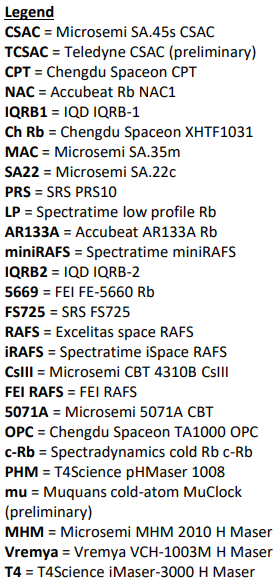
\includegraphics[width=0.83\textwidth]{img/legend.png}
            \end{figure}

        \end{column}

    \end{columns}

    \footnotetext[1]{Volume is expressed in [$cm^3$].}

\end{frame}



\begin{frame}{ADEV@1s vs. SWaP (Size, Weight and Power)}

    Similar correlation as before\footnotemark[1]: $\sigma_y(\tau=1) = 1.15 \times 10^{-10} + \text{SWaP}^{-0.27}$

    \begin{columns}[c, onlytextwidth]

        \begin{column}{0.7\textwidth}

            \begin{figure}
                \centering
                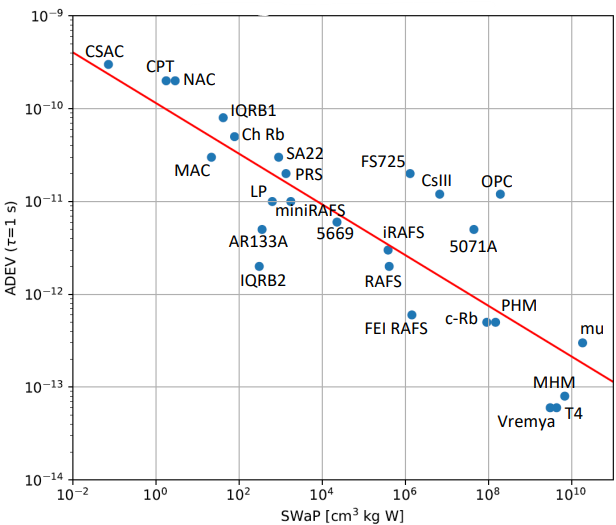
\includegraphics[width=0.9\textwidth]{img/ADEV-vs-SWaP.png}
                % \caption{Accuracy and stability of an atomic clock.}
            \end{figure}

        \end{column}

        \begin{column}{0.3\textwidth}

            \begin{figure}
                \centering
                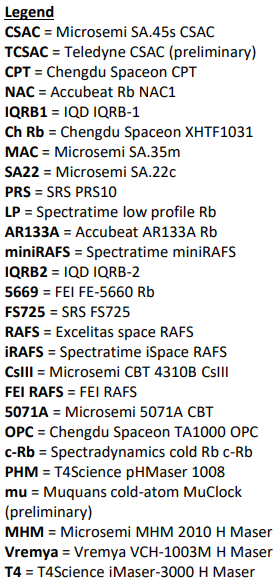
\includegraphics[width=0.83\textwidth]{img/legend.png}
            \end{figure}

        \end{column}

    \end{columns}

    \footnotetext[1]{SWaP is expressed in [$cm^3 \times kg \times W$].}

\end{frame}



\begin{frame}{Cost vs. Performance (qualitative)}

    Similar to what we have seen before, the cost of an atomic clock is proportional to its performance.

    \begin{table}
        \centering
        \resizebox{\textwidth}{!}{
            \begin{tabular}{l|llll}
                \hline
                \textbf{Technology} & \textbf{Units/year} & \textbf{Unit price} & \textbf{Worldwide sales} & \textbf{ADEV}  \\
                ~                   & ~                   & (Typical range \$)  & (\$/year)                & (1 s)          \\
                \hline
                Quartz crystals     & $5 \times 10^9$     & $[0.1; 2000]$       & $5B$                     & Low to medium  \\
                CSACs               & $12000$             & $[500; 5000]$       & $15M$                    & Medium to high \\
                Rubidium cells      & $30000$             & $[1000; 10000]$     & $150M$                   & High           \\
                Caesium beam        & $500$               & $[40000; 100000]$   & $40M$                    & Very high      \\
                Hydrogen masers     & $20$                & $>100000$           & $4M$                     & The best       \\
                \hline
            \end{tabular}
        }
        \caption{All data must be taken as indicative.}
    \end{table}

    For a CSAC, the cost is mainly driven by the packaging and assembly of the physics package.

\end{frame}
















